% !TeX root = ../main.tex
% Section 1.2.1: authentic author outputs, not a shared-method benchmark.
% Panels and exact crops are recorded in materials/literature_review/.
% Natural subfigure layout: a lettered caption above each row and images set at
% a common height, with no panel frame. Frames are reserved for structure, not
% for grouping pictures that are already aligned.
\begingroup
\linespread{1}\selectfont
\begin{tikzpicture}[
  x=1cm,y=1cm,text=black,line cap=round,line join=round,
  font=\songti\fontsize{10pt}{12pt}\selectfont,
  every node/.style={align=center,outer sep=0pt,inner sep=0pt},
  lrTitle/.style={font=\heiti\fontsize{10.2pt}{12.5pt}\selectfont},
  lrNote/.style={font=\fontsize{9.2pt}{11.5pt}\selectfont},
  lrArrow/.style={draw=black,line width=0.65pt,
    -{Latex[length=1.7mm,width=1.15mm]}}
]
  \path[use as bounding box] (0,-0.05) rectangle (16,10.35);

  % ---- (a) Shape of Motion: observation, persistent tracks, novel view ----
  \node[lrNote] at (2.725,9.60) {输入观测};
  \node[lrNote] at (8.000,9.60) {三维轨迹};
  \node[lrNote] at (13.275,9.60) {新视角重建};
  \node[anchor=north west] at (0.35,9.32)
    {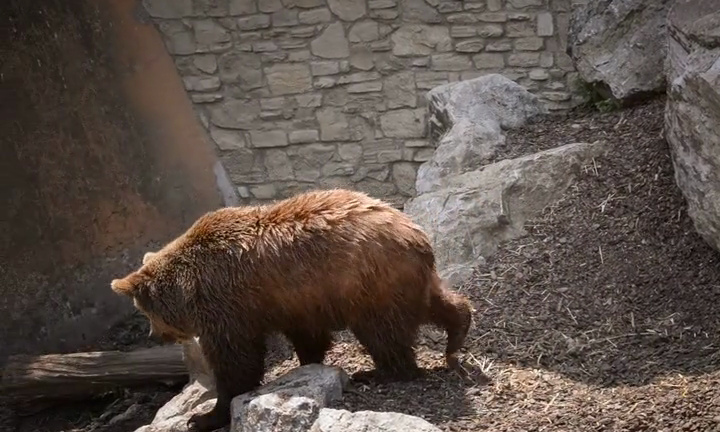
\includegraphics[width=4.75cm]{figures/generated/literature_review/som_observation.jpg}};
  \node[anchor=north west] at (5.625,9.32)
    {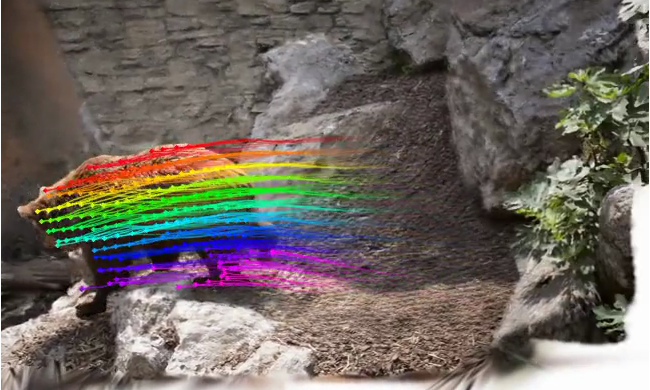
\includegraphics[width=4.75cm]{figures/generated/literature_review/som_tracks.jpg}};
  \node[anchor=north west] at (10.90,9.32)
    {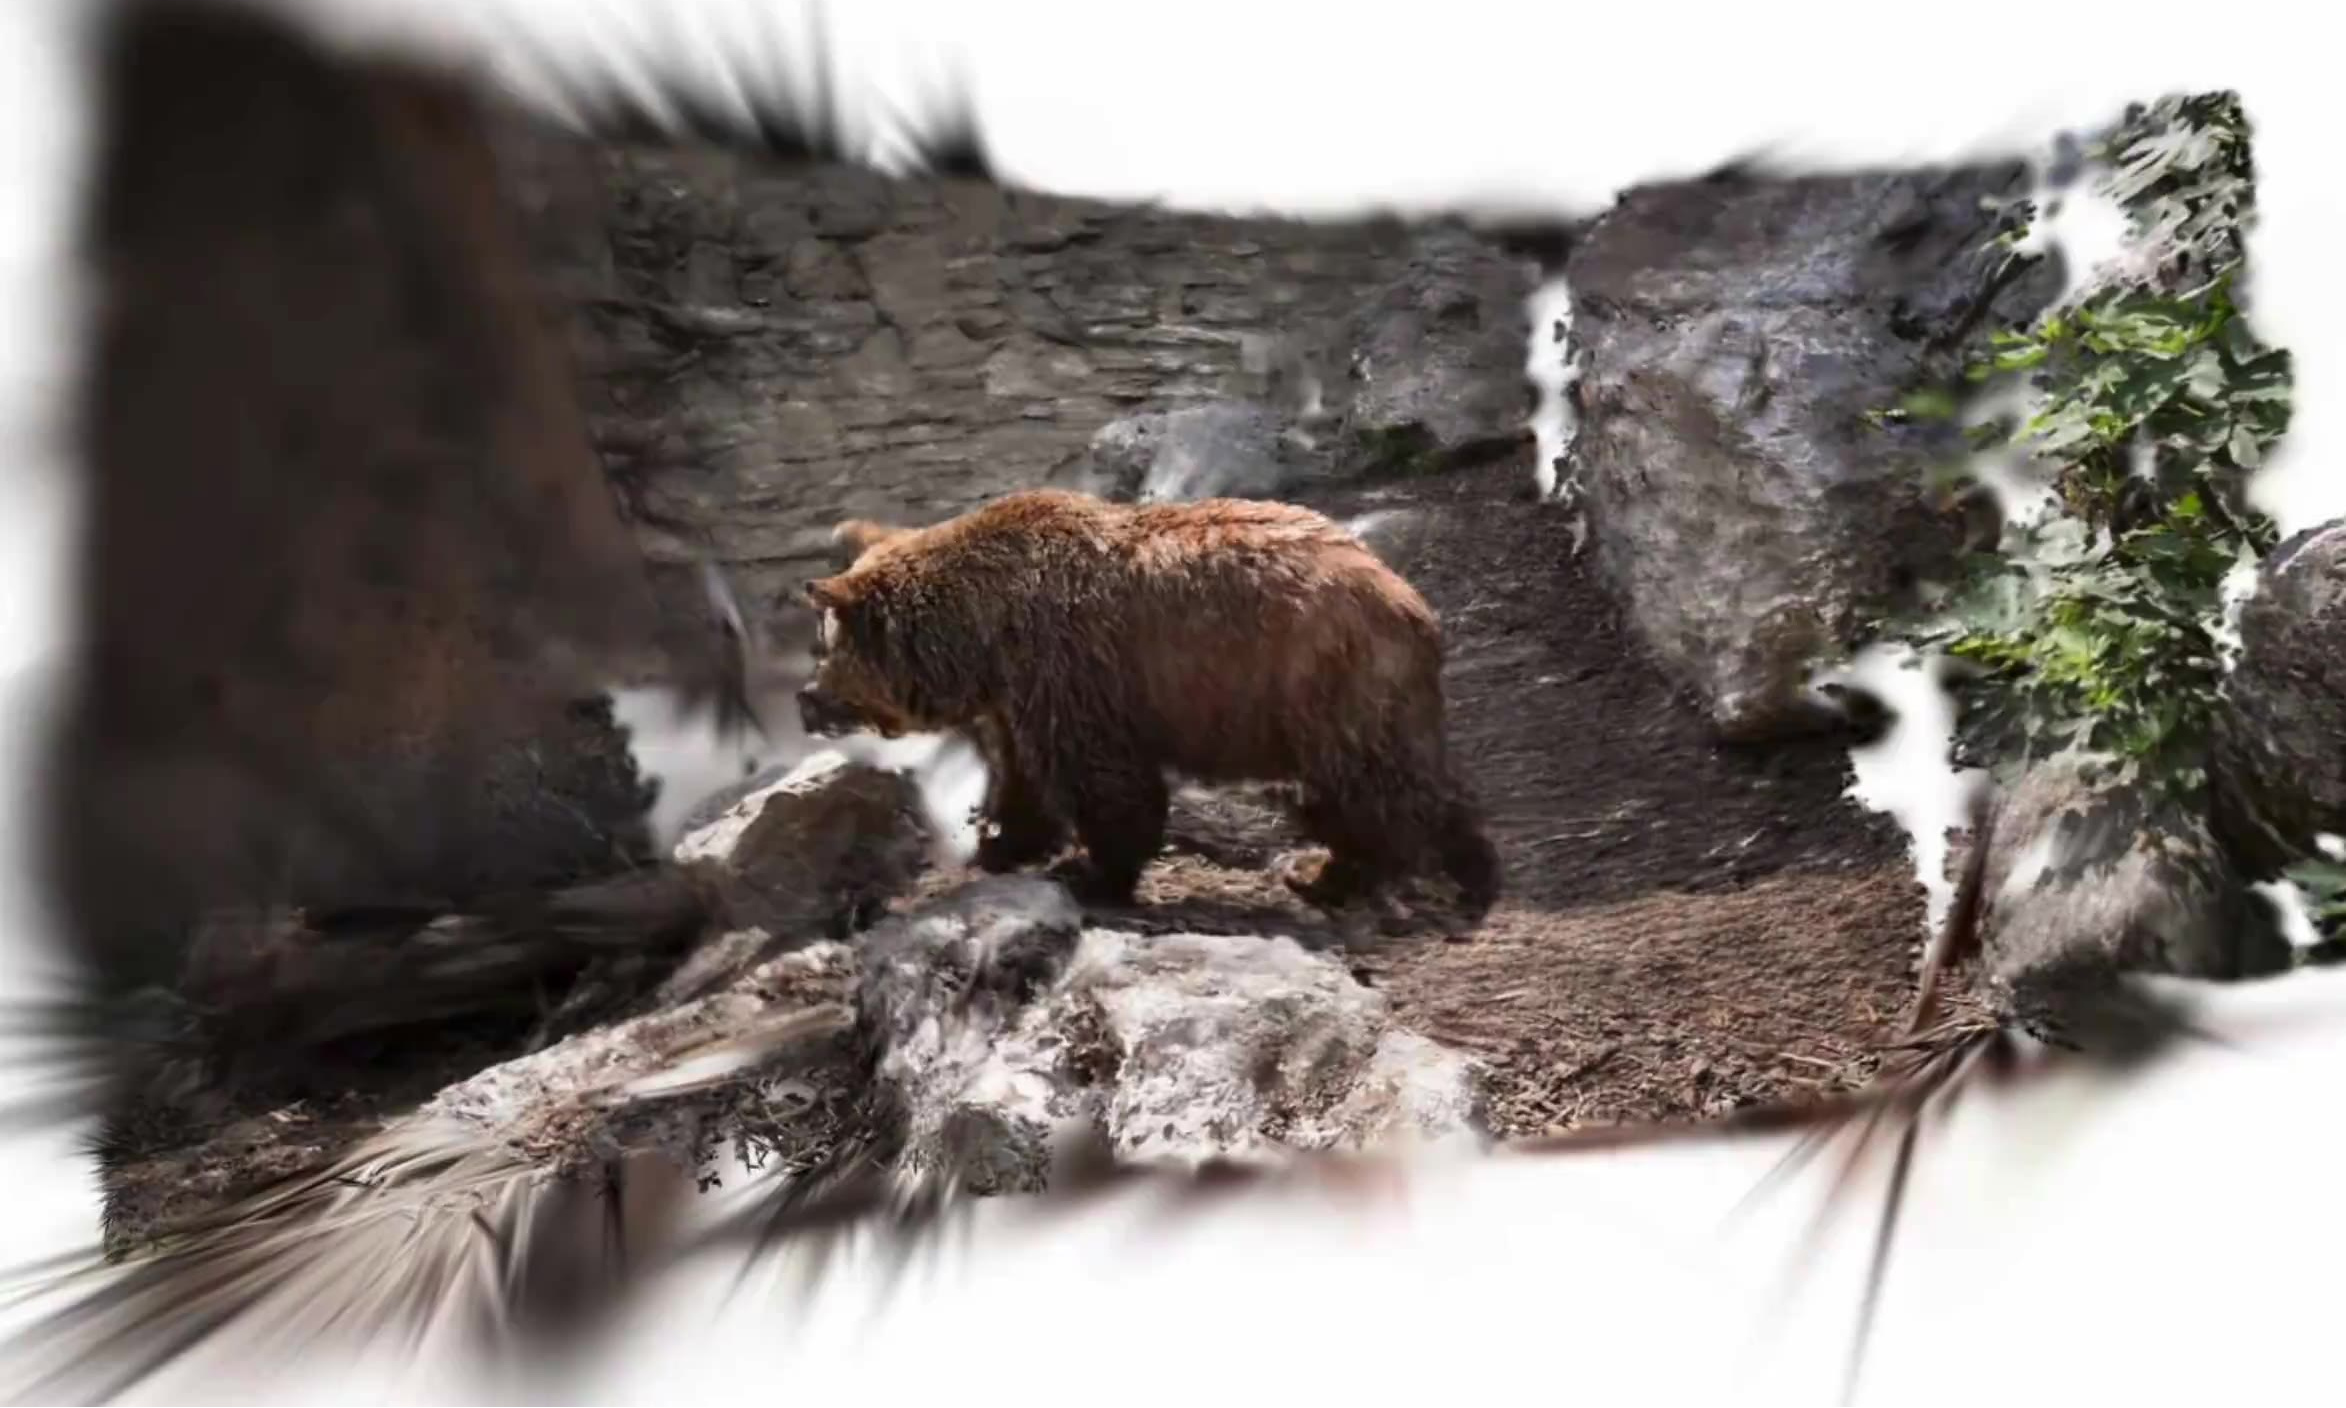
\includegraphics[width=4.75cm]{figures/generated/literature_review/som_novel_view.jpg}};
  \node[text width=7.6cm,align=center] at (8.000,6.00)
    {{\captionsetup[subfigure]{font=figsublittitle,skip=0pt}
      \subcaption{Shape of Motion}\label{subfig:lit-recon-som}}};

  \draw[black!25,line width=0.45pt] (0.10,5.66) -- (15.90,5.66);

  % ---- (b) RetimeGS: the same interval, with a non-sampled midpoint ----
  \node[lrNote] at (2.725,4.97) {采样时刻 $t_0$};
  \node[lrNote] at (8.000,4.97) {帧间时刻 $t_m$};
  \node[lrNote] at (13.275,4.97) {采样时刻 $t_1$};
  \node[anchor=north west] at (0.35,4.69)
    {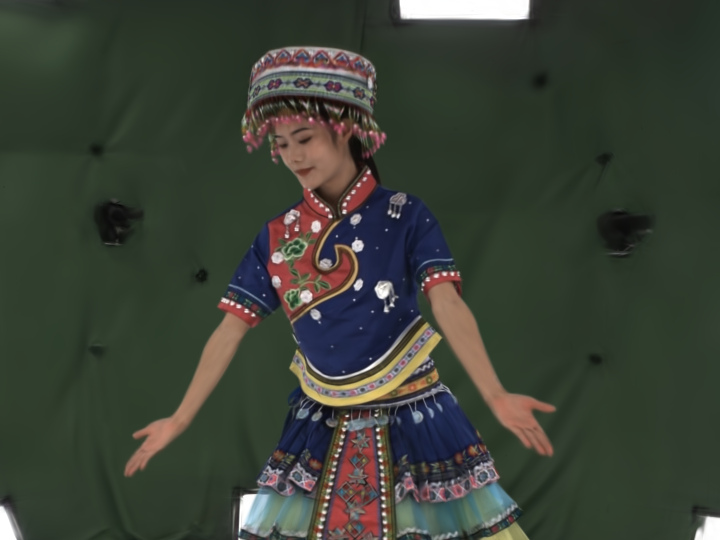
\includegraphics[width=4.75cm]{figures/generated/literature_review/retime_t0.jpg}};
  \node[anchor=north west] at (5.625,4.69)
    {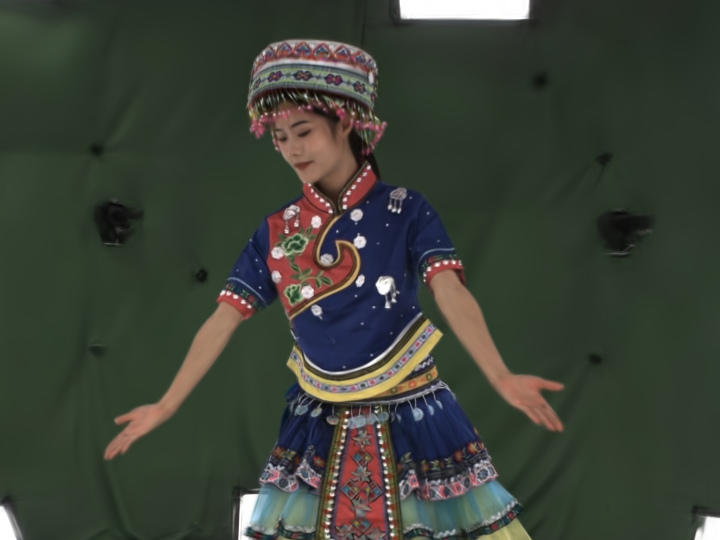
\includegraphics[width=4.75cm]{figures/generated/literature_review/retime_mid.jpg}};
  \node[anchor=north west] at (10.90,4.69)
    {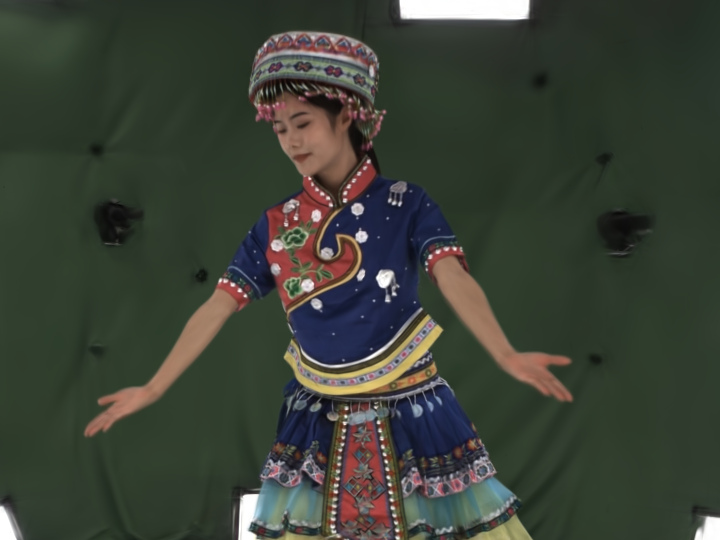
\includegraphics[width=4.75cm]{figures/generated/literature_review/retime_t1.jpg}};

  % The interval bar under the second row: sampled endpoints and the query time.
  \draw[lrArrow] (2.725,1.02) -- (13.45,1.02);
  \fill[black] (2.725,1.02) circle[radius=0.045];
  \draw[draw=black,fill=white,line width=0.7pt] (8,1.02) circle[radius=0.055];
  \fill[black] (13.275,1.02) circle[radius=0.045];
  \node[lrNote] at (8,0.72) {区间内任意时刻可查询};
  \node[text width=7.6cm,align=center] at (8.000,0.22)
    {{\captionsetup[subfigure]{font=figsublittitle,skip=0pt}
      \subcaption{RetimeGS：观测区间内插值}\label{subfig:lit-recon-retimegs}}};
\end{tikzpicture}
\endgroup
